\documentclass[conference]{IEEEtran}
\IEEEoverridecommandlockouts
% The preceding line is only needed to identify funding in the first footnote. If that is unneeded, please comment it out.
\usepackage{cite}
\usepackage[dvipsnames]{xcolor}
\usepackage{amsmath}
\usepackage{hyperref}
\usepackage{amsmath,amssymb,amsfonts}
\usepackage{algorithmic}
\usepackage{graphicx}
\usepackage{textcomp}
\usepackage{xcolor}
\def\BibTeX{{\rm B\kern-.05em{\sc i\kern-.025em b}\kern-.08em
    T\kern-.1667em\lower.7ex\hbox{E}\kern-.125emX}}
\begin{document}

\title{The Effect of Cannabis on the Brain: A Machine Learning Approach to MRI Analysis
\\
{\footnotesize \textsuperscript{}CS229 Final Project Fall 2020}
\thanks{}
}

\author{\IEEEauthorblockN{ Aaron Sossin}
\IEEEauthorblockA{\textit{(Biomedical Informatics)} \\
sosaar@stanford.edu}
\and
\IEEEauthorblockN{ Vivian Zhu}
\IEEEauthorblockA{\textit{(Biomedical Informatics)} \\
hzhu04@stanford.edu}


}

\maketitle

\begin{abstract}

Cannabis is consumed by the majority of young adults in various societies even though its health risks are relatively unknown \cite{b0}. While numerous studies have examined the effects of cannabis use on 3D anatomical brain MRIs, the use of machine learning in these analyses has been absent. This project aims at comparing the brain MRIs of heavy cannabis users and controls using machine learning techniques such as: \textit{MONAI} defined Dense CNNs, AlexNet3D, ResNet101, pretrained ResNet101 and several decoders (including \textit{NILEARN}'s SpaceNet and an SVM coupled with ANOVA). Our study supplements work done by Koenders et. al in 2016, who found that grey matter volumes of some regions were correlated to cannabis use. We find that Dense CNNs with a large amount of layers outperform famous CNN architectures like the AlexNet and ResNet that perform well on 2D classification challenges. However, further prepossessing and feature extraction is needed to obtain significant results. Although the decoders are outperformed by CNNs, they are able to isolate regions of the brain that have high predictive value to cannabis use. For example, the SVM decoder isolates the auditory system in the temporal cortex, which is consistent with the literature \cite{b5}\cite{b6}\cite{b7} and the SpaceNet decoder isolates voxels in the occipital lobe. 
\end{abstract}

%\begin{IEEEkeywords}
%Convolutional Neural Network, MRI, Cannabis, Decoder, Monai, Nilearn, Cudit, AlexNet, ResNet, SpaceNet
%\end{IEEEkeywords}

\section{Introduction}
Cannabis is only completely illegal in 6 out of 50 US states and is quickly becoming destigmatized worldwide \cite{b1}. Although it is currently the most consumed illicit drug in the world \cite{b2}, the effects of cannabis on the brain are not well understood \cite{b0}. For neuroscientists to learn about the morphological changes induced by heavy cannabis use, they often rely on Magnetic Resonance Imaging (MRI), a non-invasive procedure that creates detailed three-dimensional anatomical images \cite{b4}. Resulting images capture grey matter (GM), white matter (WM) and cerebrospinal fluid (CSF) \cite{b4}. However, neuroscientists are often unequipped to employ machine learning (ML) techniques to derive more complex MRI features. 

We suggest that applying ML to the analysis of 3D MRI scans will provide valuable insight into the brain mechanisms underlying cannabis consumption. The inputs of all our algorithms are brain MRIs, labelled by the subject’s degree of cannabis use. The output is either a classification as “control” vs. “heavy cannabis user”, or a predicted score on the Cannabis Use Disorder Identification Test (CUDIT). We propose several strategies including Convolutional Neural Networks (CNNs), transfer learning, and decoders. The CNNs comprise several \textit{MONAI} built-in DenseNets, as well as 3D versions of the AlexNet and ResNet101. The ResNet is additionally implemented with pre-trained weights derived from a kinetics video classification task. The decoders output specific voxels that have high correlations to the output, implicating specific brain regions as being effected by cannabis use. The two decoders used in this study are: 1) \textit{NILEARN}'s defined \textit{SpaceNet} and 2) a Support Vector Machine (SVM) that uses ANOVA to determine significance. At websites such as \textit{OpenNeuroCV.org} and \textit{openfmri.org}, there are a host of similarly organized datasets to the current study. These experiments should thus provide a foundation with which to explore other brain MRI research.  
%These experiments should provide a foundation with which to perform more research on open-sourced MRI databases at %websites like \url{OpenNeuroCV.org} and \url{openfmri.org}. 


\section{Related Works}

\subsection{Cannabis Use and MRI Studies
}

The literature suggests that the effects of cannabis can be seen in brain MRIs. In 2008, Yucel et. al used MRIs to find that heavy cannabis users had bilaterally reduced hippocampal and amygdala GM volumes, suggesting cannabis can lead to cell death in brain regions with a high count of endocannabinoid receptors \cite{b5}. These results were further supported by Batistella et. al in 2014 who implicated more brain regions such as the temporal and orbitofrontal cortices \cite{b6}. 

Koenders et. al published a dataset in 2016 containing T1-weighted structural Magnetic Resonance Imaging (sMRI) data \cite{b7}. In this study, Koenders et. al were primarily focused on correlating degree of cannabis use to GM volumes in select Regions of Interest (ROIs) \cite{b7}. They found GM volumes of the left hippocampus, amygdala and superior temporal gyrus to be negatively correlated with cannabis use, consistent with regions found by Yucel et. al \cite{b7}. 

Although the previous studies were effective, their research was limited to observing the GM volumes of predefined ROIs without ML. It is unlikely that this approach produces a complete description of the effects cannabis use has on the brain. CNNs should have the ability to derive more complex features such as the volumes of more flexible ROIs, the cumulative effect of several brain regions at once, and the \textit{shape} of those ROIs. In fact, researchers believe the effects of cannabis on the brain are pervasive \cite{Occipital}.

\subsection{ML applied to Medical MRIs
}

Although ML has not been used in the context of cannabis use, it has successfully examined brain MRIs in similar fields. In 2018, Zhu et. al used CNNs in conjunction with a Random Forest Classifier to predict alcohol dependence in 92 subjects \cite{b8}. In the same year, Iqbal et. al used several CNN architectures along with extensive preprocessing to accurately classify brain tumors in 220 subjects \cite{Iqbal}. This study used stochastic gradient descent (SGD) and a decaying learning rate starting at 1e-2 to train their models \cite{Iqbal}. Lu et. al used a pretrained AlexNet CNN architecture to detect pathological brain MRIs which achieved 100\% accuracy \cite{Lu}. The pretrained AlexNet outperformed the AlexNet trained from scratch\cite{Lu}. Training was done with SGD and a learning rate of 1e-4\cite{Lu}. Lerousseau et. al similarly found success in classifying brain tumors with \textit{MONAI}'s DenseNet CNN architectures, training with the Adam optimizer and learning rate of 1e-5 \cite{Lerousseau}. These studies have similar input and output to the current study, and were used to inform the methodology. 

Salvatore et. al and Moradi et. al both used extensive preprocessing with the \textit{SPM8 ToolKit} to classify brains with Parkinson's and Alzheimer's respectively \cite{b9} \cite{Moradi}. They did not use neural networks, as Moradi et. al used a voxel-based regularized logistic regression which outperformed clinician accuracy (augmented with FreeSurfer-derived features) and Salvatore et. al used Principal Component Analysis (PCA) derived features along with a SVM \cite{b9} \cite{Moradi}. These are two successful studies that highlight the power of preprocessing and data augmentation, without needing CNN architectures. 

\section{Dataset}

The data published by Koenders et. al follows the common BIDS format and is downloaded from the public repository \url{https://openneuro.org/datasets/ds000174}. Each subject is labelled as a control or heavy cannabis user and has a corresponding CUDIT score, where a higher score means heavier cannabis consumption. In all, there are 42 subjects of similar age and sex, 20 of which are considered heavy cannabis users and 22 of which are considered controls. The CUDIT scores of control subjects ($\mu{}$ = 0.11) do not exceed 1 and the scores of cannabis users ($\mu{}$ = 13.0) do not dip below 3. Each subject supplies 2 MRIs to the dataset  (one at baseline and one at a 3-year follow-up), for a total of 84 MRIs. MRIs at baseline are shape (256x182x256) and MRIs at follow up are shape (256x256x170). For reference, \textit{Fig.} 1 shows ‘sub-320’s unprocessed MRI brain scan during the follow-up session. 

In order to preprocess the MRIs, voxel intensities are normalized between 0 and 1 and the images are smoothed with a linear kernel. MRIs are also resized to the shape (96x96x96) in order to compare MRIs at the 3-year follow-up and baseline. 

\begin{figure}[htbp!]
\centerline{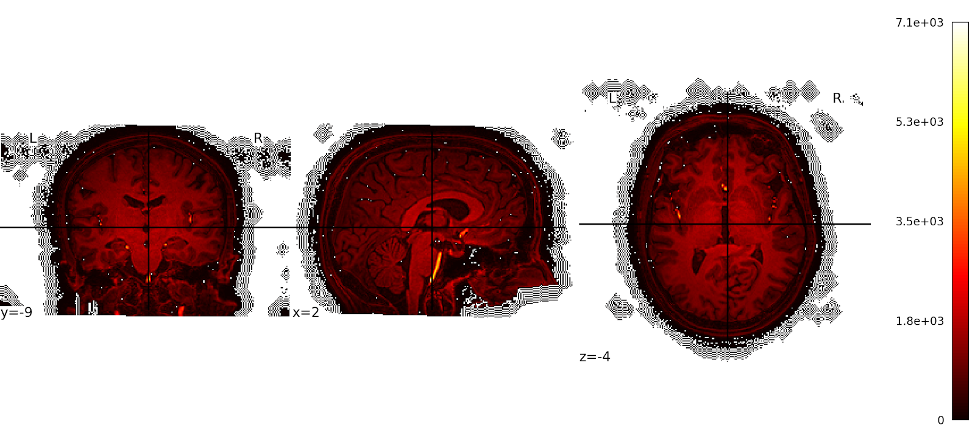
\includegraphics[scale = 0.45]{Picture2.png}}
\caption{Subject ID 320: Brain at follow-up. Color represents voxel intensity values}
\label{Picture2}
\end{figure}

\section{Methods}

\subsection{Proposed Approach
}

When testing the models' performances, evaluation score is derived from averaging across 3-fold Cross Validation (CV), where each training point is in the validation set for one run. Since the number of controls (22) vs. heavy cannabis users (20) is relatively balanced, Accuracy and Balanced Accuracy are the chosen evaluation metrics for the binary classification task. For predicting CUDIT score, Mean Squared Error (MSE) is the chosen metric.

\[Accuracy = \frac{TP + TN}{TP + TN + FP + FN} \]
\[Balanced\ Accuracy = \frac{1}{2}(\frac{TP}{TP + FN} + \frac{TN}{TN + FP}) \]
\[MSE = \frac{1}{n}\sum_{i=1}^{n}(y_{predicted} - y_{true})^{2} \]

In order to assess the best CNN implementation, a rigorous grid-search is implemented at a maximum of 50 epochs for the binary classification task. The best implementation is then tested at 200 epochs to observe its maximum score. This implementation is additionally assessed at predicting CUDIT scores. Due to time constraints, we are thus operating under the assumptions that 1) the best implementation at 50 epochs will be relatively succesful at 200 epochs, and 2) the best implementation for the binary classification task is relatively succesful at predicting CUDIT score. 

The decoders undergo the same 3-fold CV during their training and validation phases for each task. However, when producing maps that isolate the voxels with the highest statistical power, they are fit to the entire dataset. 



\subsection{MONAI defined DenseNet Architectures}

\textit{MONAI} is a PyTorch based deep learning open-source framework that supports analyzing MRI files of the format “.nii.gz” \cite{MONAI}. \textit{DenseNet121}, \textit{DenseNet169} and \textit{DenseNet264} are three densely connected CNNs with 121, 169 and 264 layers respectively. They are specified by the \textit{monai.nets.densenet} module. Dense CNNs connect each layer to every other layer in a feed-forward fashion. They are known to strengthen feature propagation and reduce the number of parameters needed to train the model, decreasing susceptibility to overfitting \cite{Huang}. One of the inspirations for their creation was the redundancy found in similar ResNet architectures \cite{Huang}. 

A grid-search inspired by the Related Works section is utilized to find the optimal hyper-parameters for distinguishing controls from heavy cannabis users in the binary classification task. If not for time constraints, a more extensive grid-search would be executed. This task is run on the Google Cloud Platform and takes advantage of \textit{CUDA}. \textit{Table} 1 outlines the results. 

\begin{itemize}
    \item Learning Rates: [1e-3, 1e-5]
    \item Optimizers: [Adam, SGD]
    \item Loss Function: Cross Entropy Loss
    \item Max #Epochs: 50
\end{itemize}


\subsection{Classically Successful CNN Architectures: AlexNet and ResNet}

AlexNet is a famous CNN architecture that in 2012 dramatically improved results on the ImageNet Large Scale Visual Recognition Challenge (ILSVRC) \cite{Alom}. AlexNet3D is Alex Krizhevsky’s 2012 implementation with 3D convolutional layers and can be found at: https://github.com/denti/AlexNet3D. AlexNet3D has 5 convolutional layers and 3 fully connected layers. This implementation thus has far fewer layers and weights than the DenseNets.

Residual Networks (ResNets) have similarly performed well on the ILSVRC \cite{Data}. The specific implementation used in this report can be found at https://github.com/Tushar-N/pytorch-resnet3d/blob/master/models/resnet.py. We use ResNet101 with 101 layers.

Transfer learning conceptually seeks to improve performance on a task through the incorporation of previously assembled knowledge from similar tasks. In the context of CNNs, this often involves the use of pretrained models with saved weight parameters. This supplies a "better-than-random" starting point and allowed Lu et. al to improve their detection of pathological brain MRIs as previously mentioned \cite{Lu}. In our case, the ResNet CNN architecture is experimented with and without pretrained weights from a kinetics task that classifies videos.

The same exact grid-search was performed on the above networks as for the \textit{MONAI} defined DenseNets, the results of which can similarly be seen in \textit{Table} 1. 




\subsection{Decoders: SpaceNet and SVM}

\textit{NILEARN} leverages the \textit{Sklearn} toolbox \cite{SKLEARN} and is a Python module for analyzing NeuroImaging data. \textit{NILEARN}’s api resamples the images to the MNI-152 template, as well as smooths and standardizes the images using the \textit{NiftiMasker} function. Both decoders undergo 3-fold CV to assess scores in the binary classification task and CUDIT prediction task. 

The first decoder is \textit{Sklearn}’s implementation of SVM with a linear kernel that works in conjunction with ANOVA tests to determine the statistical importance of each voxel, where the top 5\% are selected. \textit{Sklearn}
s default settings are used. 

The \textit{SpaceNetClassifier} and \textit{SpaceNetRegressor} are built-in models from \textit{NILEARN} that use a multivariate method for brain decoding and segmentation. These SpaceNets can implement two spatial penalties that help improve brain decoding power: "graph-net" and "tv-l1". 

\textit{Fig.}2 reveals the most predictive voxels isolated by the decoders. \textit{NILEARN}'s \textit{plot\_stat\_map} function is used to generate the figures. The predictive voxels are highlighted and overlayed on top of a representation of the average MRI across the dataset calculated using the \textit{nilearn.image.mean\_img} function. Absolute value of weight reveals a voxel’s predictive value, while positive (red-ish) vs. negative (blue-ish) sign determines the direction of this correlation; a higher or lower voxel intensity may correlate with more or less cannabis use.


\begin{figure}[htbp]
%\centerline{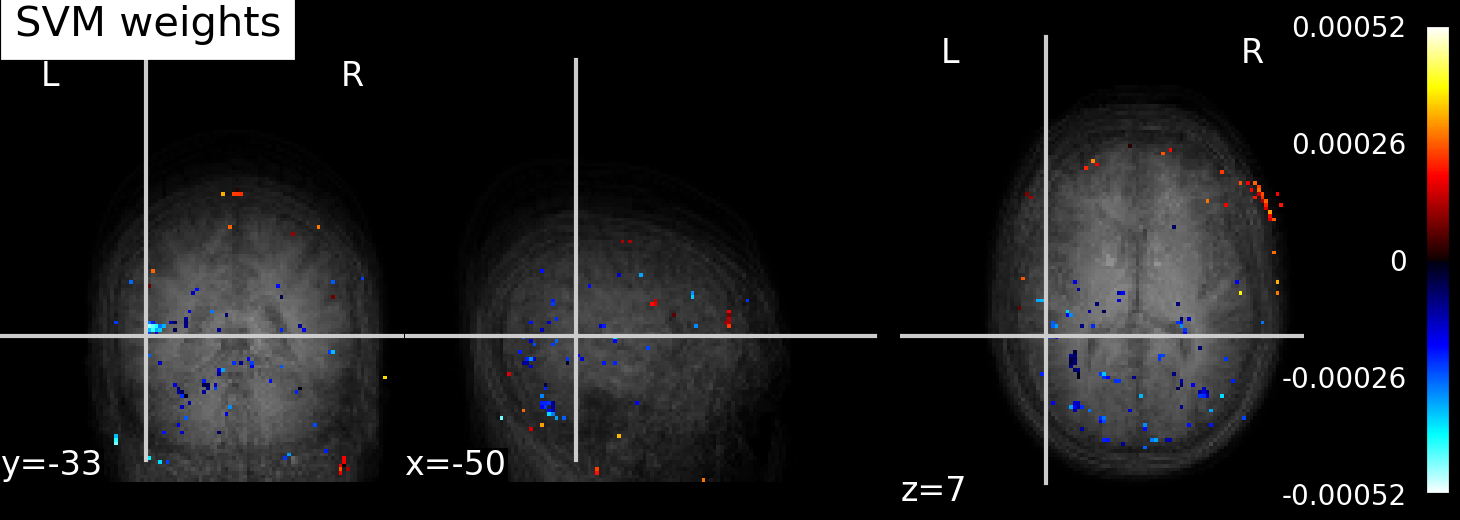
\includegraphics[scale = 0.45]{svm_decoding.png}}
%\centerline{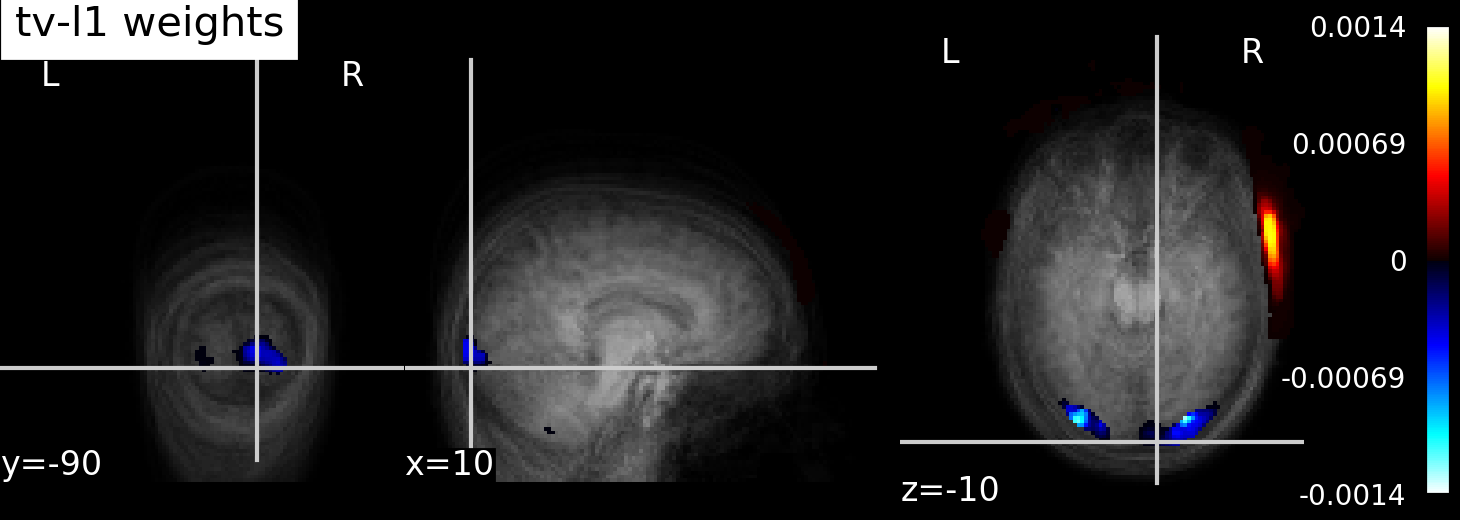
\includegraphics[scale = 0.45]{tv-l1BESTBEST.png}}
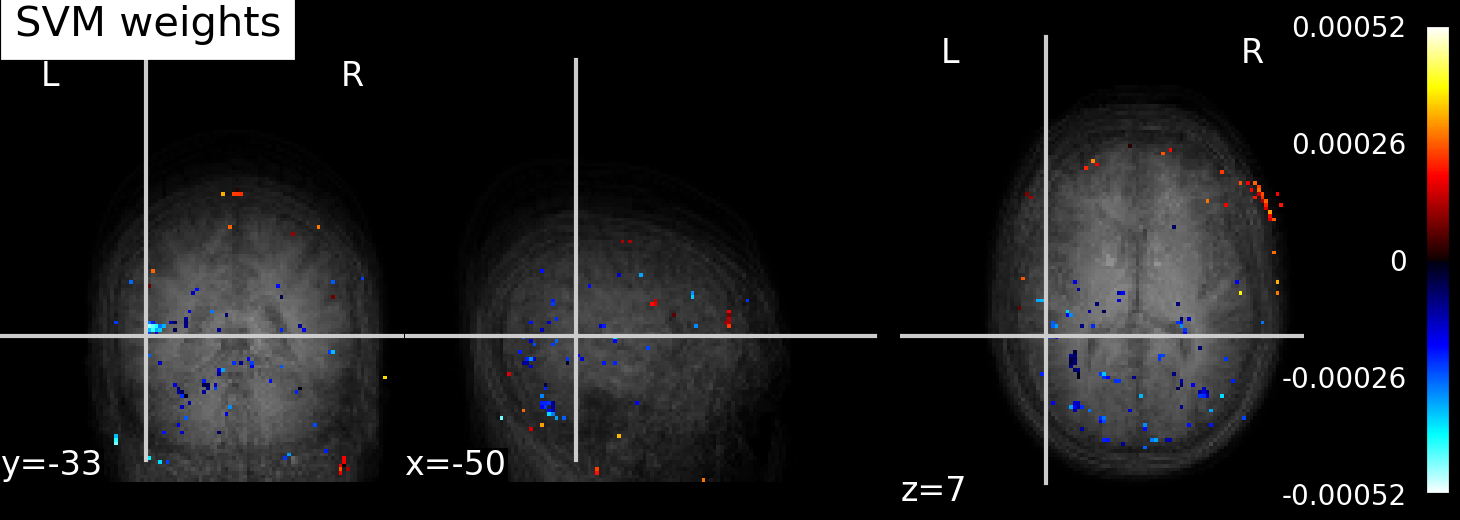
\includegraphics[scale=0.45]{svm_decoding.png} \\ \\
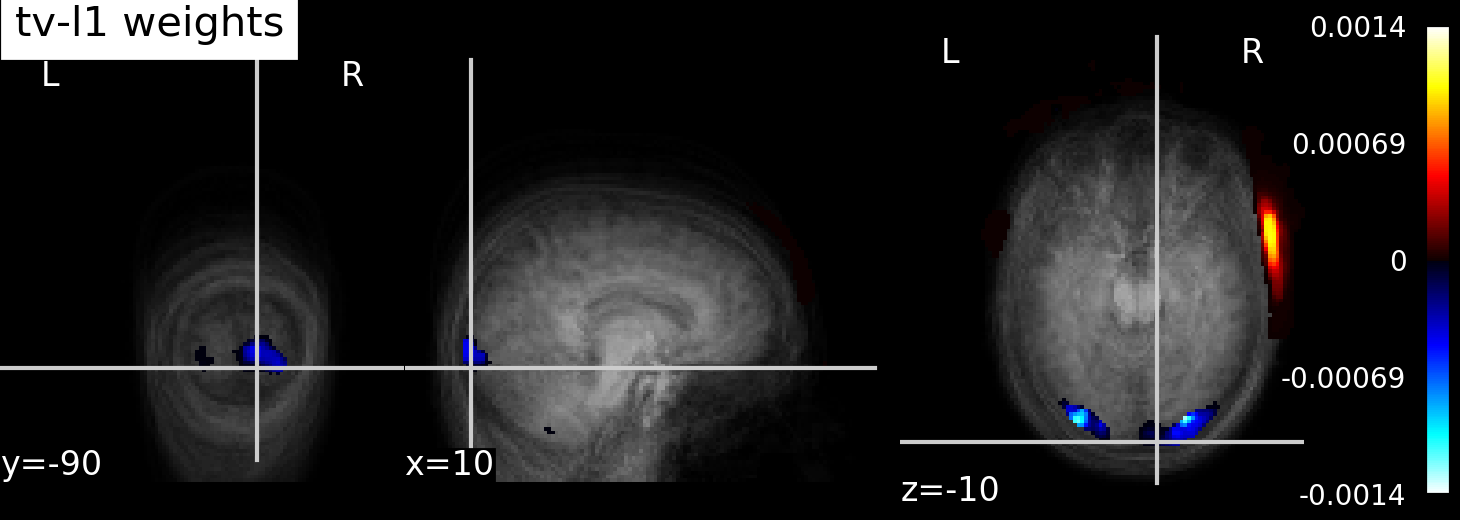
\includegraphics[scale=0.45]{tv-l1BESTBEST.png}
\caption{Decoded Voxels: SVM during binary classification (top), SpaceNet with "tv-l1" penalty during CUDIT Score Prediction (bottom)}
\label{Picture1}
\end{figure}


\begin{table}[Classification]
\caption{Binary Classification of MRIs as Controls or Heavy Cannabis Users}
\begin{center}
\begin{tabular}{|p{1.5cm}|c|c|c|}
\hline

\cline{2-4} 
\textbf{Model Type} & \textbf{\textit{Hyper-parameters}}& \textbf{\textit{Accuracy}}& \textbf{\textit{Balanced Accuracy}} \\
\hline

\multirow{DenseNet121} 
& Adam, 1e-3 & 0.61 & 0.60 \\ 
& Adam, 1e-5 & 0.67 & \color{PineGreen}0.65 \\ 
& SGD, 1e-3 & 0.59 & 0.60 \\
& SGD, 1e-5 & 0.64 & 0.55 \\

\hline

\multirow{DenseNet169} 
& Adam, 1e-3 & \color{PineGreen} 0.68 & 0.57 \\ 
& Adam, 1e-5 & 0.60 & 0.59 \\ 
& SGD, 1e-3 & 0.61 & 0.57 \\
& SGD, 1e-5 & \color{BrickRed}0.40 & 0.52 \\

\hline

\multirow{\color{PineGreen}DenseNet264} 
& Adam, 1e-3 & 0.60 & 0.61 \\ 
& Adam, 1e-5 & 0.66 & \color{PineGreen}0.65 \\ 
& SGD, 1e-3 & 0.58 & 0.59 \\
& SGD, 1e-5 & 0.61 & 0.61 \\

\hline

\multirow{AlexNet3D} 
& Adam, 1e-3 & 0.57 & 0.57 \\ 
& Adam, 1e-5 & 0.57 & 0.57 \\ 
& SGD, 1e-3 & 0.50 & 0.50 \\
& SGD, 1e-5 & 0.53 & 0.51 \\

\hline

\multirow{ResNet101} 
& Adam, 1e-3 & 0.50 & 0.50 \\ 
& Adam, 1e-5 & 0.53 & 0.51 \\ 
& SGD, 1e-3 & 0.52 & 0.52 \\
& SGD, 1e-5 & 0.53 & 0.50 \\

\hline
\multirow{Pretrained ResNet101}
& Adam, 1e-3 & 0.55 & 0.54 \\ 
& Adam, 1e-5 & 0.58 & 0.60 \\ 
& SGD, 1e-3 & 0.52 & 0.51 \\
& SGD, 1e-5 & 0.52 & 0.51 \\

\hline

\multirow{\color{BrickRed}SpaceNet} 
& graph-net penalty & 0.51 & \color{BrickRed}0.46 \\ 
& tv-l1 penalty & 0.46 & 0.50 \\ 

\hline

\multirow{SVM} 
& - & 0.52 & 0.53 \\ 

\hline



\multicolumn{4}{l}{}
\end{tabular}
*Scores represent the average maximum accuracy across 3-fold CV and that epoch's corresponding balanced accuracy score
\label{tab1}
\end{center}
\end{table}
%Scores represent the average maximum accuracy across %3-fold CV and that \newline
%epoch's corresponding balanced accuracy score


\subsection{Identifying Predictive Brain Regions
}

Since images are resampled to the MNI-152 reference affine, the (x,y,z) coordinates refer to documented brain regions. The voxels of highest predictive value according to the SVM are clustered around the coordinates (-50, -33, 7) as shown in \textit{Fig. }2. These coordinates are input into \textit{Neurosynth}’s “Locations” software \cite{Neurosynth} which isolates the auditory cortex (in the temporal lobe) as belonging to these coordinates. The same process is applied to the SpaceNet derived coordinates of (10, -90,-10) which corresponds to the occipital lobe. The penalty term did not significantly effect the identified voxels and so only the tv-l1 is shown in \textit{Fig.}2. 

\subsection{Best Implementation at 200 Epochs}

Based on \textit{Table} 1, DenseNet264 performs the best during the 3-fold cross validated grid-search. \textit{Fig.} 3 shows the result of this implementation tested at 200 epochs with the same parameters. In \textit{Fig.} 3, the left y-axis denotes the average training loss per epoch while the right y-axis denotes the classification accuracy at a specific epoch tested against the validation set. \textit{Table} 2 describes the results. 


\begin{figure}[hb]
\centerline{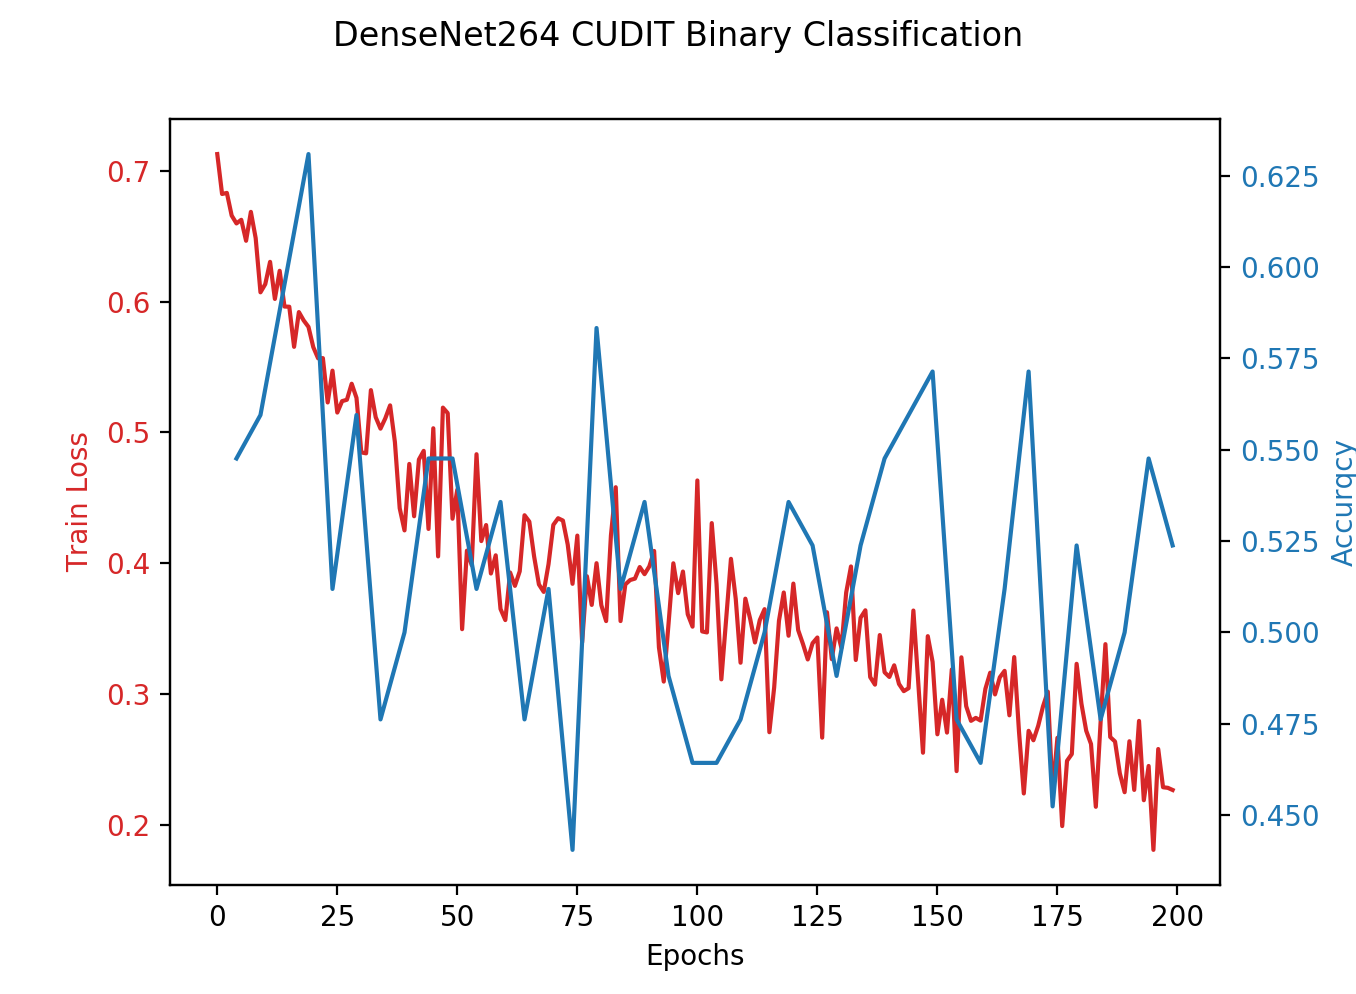
\includegraphics[scale = 0.50]{binary_200.png}}
\caption{Binary Classification Training. Average values across 3-fold CV shown.}
\label{Picture1}
\end{figure}


\begin{table}[htb]
\caption{DenseNet264 Binary Classification Results at 200 Epochs}

\begin{center}
\begin{tabular}{|c|c|c|c|}
\hline

\cline{2-4} 
\textbf{Accuracy} & \textbf{\textit{Balanced Accuracy}}& \textbf{\textit{Sensitivity}}& \textbf{\textit{Specificity}} \\
\hline

\multirow{0.67} 
& 0.67 & 0.61 & 0.73 \\ 

\hline

\multicolumn{4}{l}{}
\end{tabular}

*Scores represent the average maximum accuracy across 3-fold CV and that epoch's other metrics
\label{tab1}
\end{center}
\end{table}





\subsection{Predicting CUDIT Score}

In order to predict CUDIT scores, the output layer of the DenseNet264 is changed from size 2 to 30. \textit{Fig.} 4 and \textit{Fig.} 5 show the results of this implementation, while \textit{Table} 2 shows the success of several models at this task. 

\begin{figure}[h]
\centerline{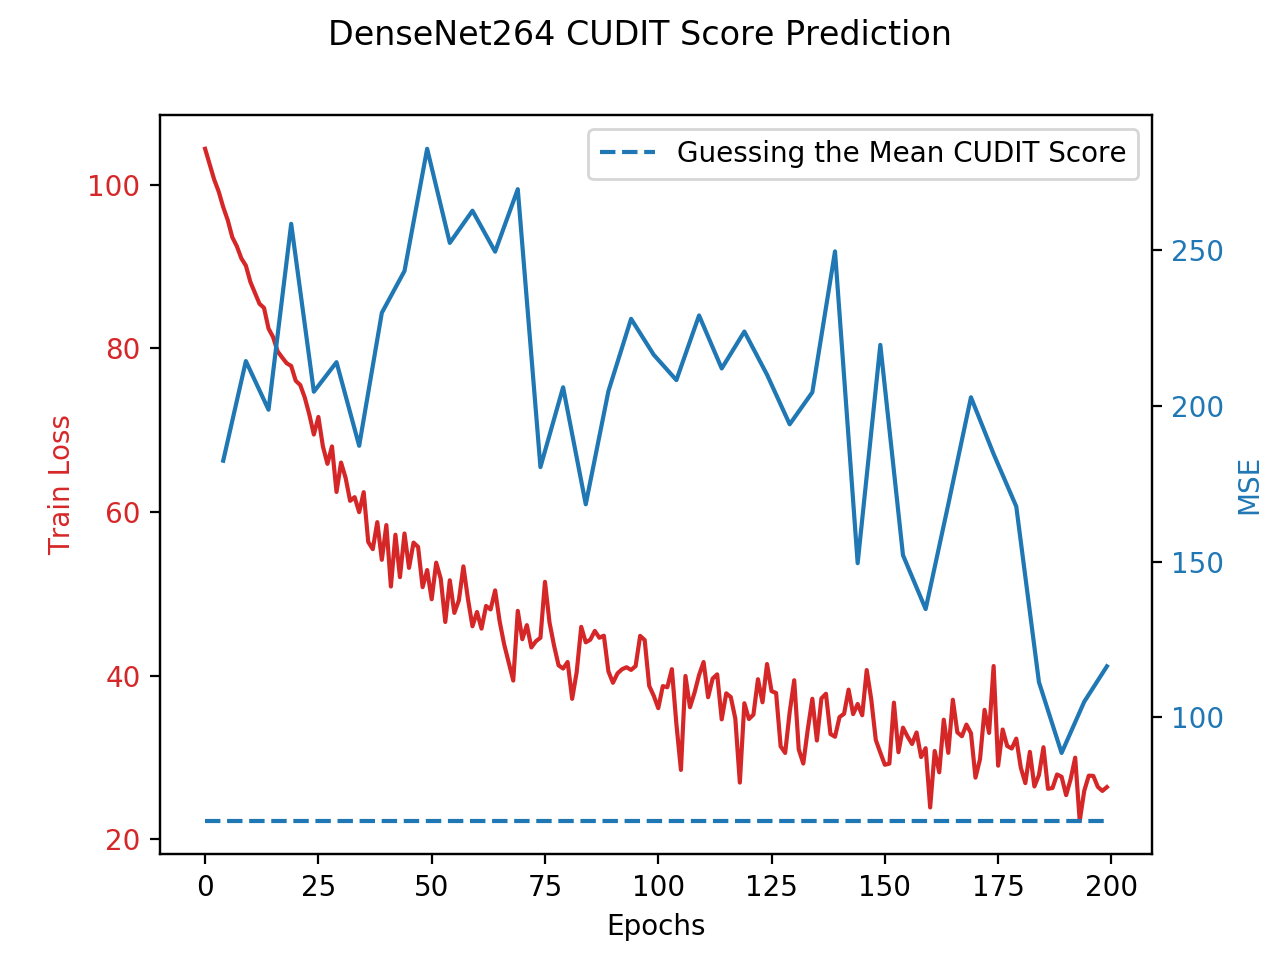
\includegraphics[scale = 0.45]{DenseNet264_CuditScorePrediction_TrainLoss.png}}
\caption{CUDIT Score Prediction during Training. Average values across 3-fold CV shown. }
\label{Picture1}
\end{figure}

\begin{figure}[h]
\centerline{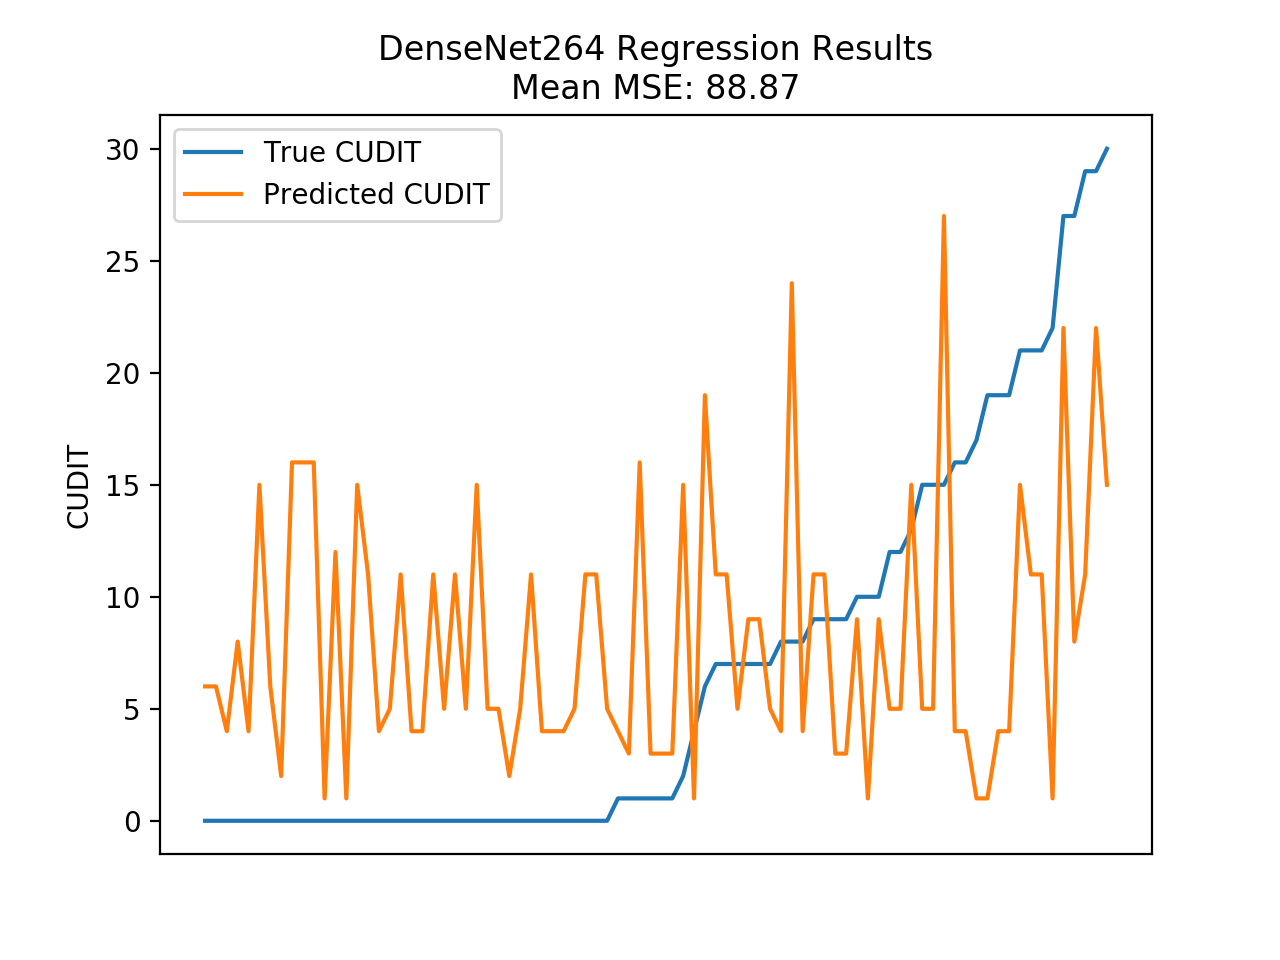
\includegraphics[scale = 0.45]{DenseNet264_CuditScorePrediction_Visual.png}}
\caption{CUDIT Score Prediction Results. Average values across 3-fold CV shown.}
\label{Picture1}
\end{figure}

\begin{table}[htbp]
\caption{CUDIT Score Prediction Results}

\begin{center}
\begin{tabular}{|c|c|}
\hline

\cline{2-4} 
\textbf{Model} & \textbf{\textit{MSE}} \\
\hline

\multirow{\color{PineGreen}DenseNet264} 
& \color{PineGreen}89 \\ 

\hline

\multirow{SpaceNet w/ graph-net} 
& 105 \\ 

\hline

\multirow{\color{BrickRed}SpaceNet w/ tv-l1} 
& \color{BrickRed}112 \\ 

\hline

\multirow{SVM} 
& 99 \\ 

\hline

\multicolumn{4}{l}{}
\end{tabular}
\label{tab1}
\end{center}
\end{table}




\section{Discussion
}

\subsection{Controls vs. Heavy Cannabis Users
}

The DenseNets outperform all other implementations during the 50 epoch grid-search. Not only do the DenseNets comprise the best implementations, but they are more consistent across different hyperparameters (\textit{Table} 1). Although the DenseNets perform similarly to each other, DenseNet264 with the Adam optimizer and 1e-5 learning rate is the best implementation with accuracy 66\% and balanced accuracy 65\% (\textit{Table} 1). When run for 200 epochs, this implementation slightly improves to an accuracy across 3-fold cross validation of 67\% and balanced accuracy 67\% (\textit{Table} 2). However, \textit{Fig}. 3 reveals that accuracy does not generally improve in the later epochs. Amongst the decoders, the SVM implementation performs the best with an accuracy of 52\% and balanced accuracy of 53\% (\textit{Table} 1). 

Although the pretrained ResNet101 was trained on a kinetics task (quite dissimilar to the proposed MRI classification task), it still slightly improves accuracy (from 0.53\% to 0.58\%) and balanced accuracy (from 0.52\% to 0.60\%) (\textit{Table} 1). Should learning be transferred from another MRI classification task, we suspect results would improve even more. 

There is evidence to suggest both overfitting and underfitting by the CNNs. As the number of layers increase in a model, so do the number of weights that are being learned and the potential for unnecessary complexity. The fact that the DenseNet with the most layers (DenseNet264) outperforms other DenseNets in the 50-epoch grid-search suggests that the training data is not being overfit in the beginning. However, \textit{Fig.} 3 shows that as epochs continue to increase, the DenseNet264's accuracy does not improve - likely due to overfitting. This puts the assumption that relative success in the grid-search holds at 200 epochs into question; a smaller model may overfit less, and improve better with more epochs. 

The AlexNet has far fewer layers than the DenseNet and ResNets, which may explain its shortcomings at classifying the MRIs. However, the ResNet has the highest complexity of all the models and also performs worse than the DenseNets in the 50-epoch grid-search. These results suggest that classically succesful CNN architectures on the ILSVRC are less well suited to analyze 3D MRIs than denser CNNs architectures with many layers.


\subsection{Predicting CUDIT Score}

DenseNet264 outperforms the decoders at predicting CUDIT scores with an MSE of 88.87. However, this is not significant since constantly guessing the average CUDIT score of 6.4 yields a 66.83 MSE. \textit{Fig.} 4 shows improvement over training with respect to average train loss and MSE, which suggests that this model is not overfitting the training data. Since convergence was not yet achieved, more epochs may have improved MSE and this can be improved. \textit{Fig.} 5 highlights the model's struggle to predict CUDIT score. It is also worth testing the assumption that the best model at binary classification holds for this task with a separate grid-search.

\subsection{Identifying Predictive Brain Regions}

Neither decoder is particularly successful, meaning that the isolated voxels need to be contemplated with skepticism. As previously stated, the voxels identified by the SVM correspond to the auditory system, which lies in the temporal cortex. This brain region also important for memory \cite{Receptors} is consistent with other cannabis studies that implicate the temporal cortex \cite{b5}\cite{b6}\cite{b7}. Furthermore, this brain region is known to have endocannabinoid receptors \cite{Receptors}, making it a reasonable area to find high predictive value. The SpaceNet decoders isolate voxels in the occipital lobe, which is principally implicated in visual processing. Although this is not a brain region classically connected to cannabis use, the brain effects of cannabis may be present throughout the brain \cite{Occipital}.

\subsection{Improvements to the Current Study}

There are several ways the current study can be improved. Further preprocessing the MRI images beyond smoothing and normalizing would be a good first step. Moradi et. al and Salvatore et. al found success in using the \textit{SPM8} preprocessing package which includes skull-stripping, cropping, etc... \cite{Moradi} \cite{b9}. Further preprocessing has not only the potential to improve results, but can easily fit within the pre-existing code base. There are also data augmentation techniques which can be incorporated. Salvatore et. al used PCA to extract features from the MRIs \cite{b9}, and Moradi et. al proved the efficacy of using \textit{FreeSurfer} derived features such as thickness estimations, volumetric segmentation, inter-subject alignments, etc... \cite{FreeSurfer} \cite{Moradi}. A Random Forest classifier could combine the output of CNNs and these extracted features. 

Since transfer learning classically improves scores \cite{Lu} including our ResNet101 model, and large Dense CNNs are succesful, we predict that large dense CNNs that were previously trained on MRI analysis tasks pose the ideal model type to continue research. 



\section{Conclusion}

%{A comprehensive overview of several strategies was conducted to distinguish the brains of cannabis users and controls. CNNs, transfer learning, and decoders were successfully implemented in this analysis, where Monai’s built-in DenseNet264 had the most success at 50 epochs with classification accuracy at \%. This approach at 200 epochs showed X improvement to an accuracy of \%. The most succesful decoder was the SVM and ANOVA implementation which garnered a classification accuracy of and a regression MSE of Y. This decoder isolated the J and X brain regions as having voxels of high predictive value. These regions are known to have endocannabinoid receptors, thus showing consistency with the literature. In order to improve the MRI analysis, further pre-processing needs to be performed, including augmenting the dataset with FreeSurfer derived features. The results do not display an overwhelming ability to determine cannabis use from brain MRIs, but provides a solid foundation with which to continue research in this area. The repository also lays out a pipeline for conducting other sMRI studies in the OpenNeuroCV database. }


Several strategies were implemented to try and differentiate MRIs from subjects of varying cannabis use. The dense CNN architectures with large number of layers tended to outperform classically succesful models on the ILSVRC 2D classification challenge and decoders. The highest achieved accuracy at distinguishing cannabis users from controls was 67\% and the lowest MSE at predicting CUDIT scores was 88.87, neither of which are significant results. The SVM decoder identified voxels in the temporal cortex as being the most predictive which is consistent with the literature \cite{b5}\cite{b6}\cite{b7}. Alternatively, the SpaceNet decoders isolated regions in the occipital lobe. This study successfully implemented DenseNets, AlexNet, ResNet, transfer learning and several decoders to analyze brain MRIs.
There are several classically effective preprocessing and data augmentation strategies that can supplement this research. The methods outlined in this study and the attached GitHub repo can help inform future brain MRI studies that are inherently similar.

\section*{Code}
GitHub link can be found at \url{https://github.com/aaronsossin/Cannabis-MRI-Machine-Learning}. More details about the code are found there. 

\section*{Contributions}

Aaron S. and Vivian Z. contributed equally to every aspect of this project.




\begin{thebibliography}{00}

\bibitem{b1} “Map of Marijuana Legality by State.” DISA Global Solutions, 9 Nov. 2020, disa.com/map-of-marijuana-legality-by-state
\bibitem{b2} 1. Degenhardt L, Hall W (2012): Extent of illicit drug use and dependence, and their contribution to the global burden of disease. The Lancet 379:55–70
\bibitem{b0} Hall, W. A. Y. N. E., L. L. O. Y. D. Johnston, and N. E. I. L. Donnelly. "Epidemiology of cannabis use and its consequences." The health effects of cannabis (1999): 71-125.
\bibitem{b4} Blink, Evert J. "mri: Physics." Online PDF file (2004): 0-75.
\bibitem{b5} Yücel, Murat, et al. "Regional brain abnormalities associated with long-term heavy cannabis use." Archives of general psychiatry 65.6 (2008): 694-701.
\bibitem{b6} Battistella, Giovanni, et al. "Long-term effects of cannabis on brain structure." Neuropsychopharmacology 39.9 (2014): 2041-2048.
\bibitem{b7} Koenders, Laura, et al. "Grey matter changes associated with heavy cannabis use: a longitudinal sMRI study." PLoS One 11.5 (2016): e0152482.
\bibitem{Occipital} Rais, Monica, et al. "Cannabis use and progressive cortical thickness loss in areas rich in CB1 receptors during the first five years of schizophrenia." European Neuropsychopharmacology 20.12 (2010): 855-865.
\bibitem{b8} Zhu, Xi, et al. "Random forest based classification of alcohol dependence patients and healthy controls using resting state MRI." Neuroscience letters 676 (2018): 27-33.
\bibitem{Iqbal} Iqbal, Sajid, et al. "Brain tumor segmentation in multi‐spectral MRI using convolutional neural networks (CNN)." Microscopy research and technique 81.4 (2018): 419-427.
\bibitem{Lu} Lu, Siyuan, Zhihai Lu, and Yu-Dong Zhang. "Pathological brain detection based on AlexNet and transfer learning." Journal of computational science 30 (2019): 41-47.
\bibitem{Lerousseau} Lerousseau, Marvin, Eric Deutsh, and Nikos Paragios. "Multimodal brain tumor classification." arXiv preprint arXiv:2009.01592 (2020).
\bibitem{b9} Salvatore, Christian, et al. "Machine learning on brain MRI data for differential diagnosis of Parkinson's disease and Progressive Supranuclear Palsy." Journal of neuroscience methods 222 (2014): 230-237.
\bibitem{Moradi} Moradi, Elaheh, et al. "Machine learning framework for early MRI-based Alzheimer's conversion prediction in MCI subjects." Neuroimage 104 (2015): 398-412.
\bibitem{MONAI} Jungo, Alain, et al. "pymia: A Python package for data handling and evaluation in deep learning-based medical image analysis." Computer Methods and Programs in Biomedicine (2020): 105796.

\bibitem{Huang}Huang, Gao, et al. "Densely connected convolutional networks." Proceedings of the IEEE conference on computer vision and pattern recognition. 2017.
\bibitem{Alom} Alom, Md Zahangir, et al. "The history began from alexnet: A comprehensive survey on deep learning approaches." arXiv preprint arXiv:1803.01164 (2018).




\bibitem{Data} Tsang, Sik-Ho. “Review: DenseNet - Dense Convolutional Network (Image Classification).” Medium, Towards Data Science, 20 Mar. 2019, towardsdatascience.com/review-densenet-image-classification-b6631a8ef803. 
\bibitem{SKLEARN} Buitinck, Lars, et al. "API design for machine learning software: experiences from the scikit-learn project." arXiv preprint arXiv:1309.0238 (2013).
\bibitem{Neurosynth} “(0, 0, 0).” Neurosynth, www.neurosynth.org/locations/. 
\bibitem{Receptors} Rocha, Luisa, et al. “Endocannabinoid System and Cannabinoid 1 Receptors in Patients With Pharmacoresistant Temporal Lobe Epilepsy and Comorbid Mood Disorders.” Frontiers in Behavioral Neuroscience, Frontiers Media S.A., 6 May 2020, www.ncbi.nlm.nih.gov/pmc/articles/PMC7218130/. 

\bibitem{FreeSurfer} Fischl, Bruce. "FreeSurfer." Neuroimage 62.2 (2012): 774-781.


\end{thebibliography}


\vspace{12pt}


\end{document}
